%% specs
%% 2007 Eiji Fukutomi
この章では,各実験で満たすべき最低限の仕様を述べる.
基本実験と応用実験それぞれに対して,目的と内容および考慮すべき事項についておおまかに書いている.
ただし,\textbf{\Underline{このように}}下線と強調文字で書かれている部分は,さらに補足説明が必要である.
レポートなどに利用するときには\textbf{\Underline{適宜}}各自で説明を加えること.

\vspace{-1zh}
\section{第1回 OSのインストール}

パーソナルコンピュータ(PC)およびワークステーション(WS)は、一切ソフ
トウェアが入っていない状態では,ユーザに対して計算や通信といった機能を
提供することができない.本実験ではまず,これらPCやWSの機能を,ユーザ
が\textbf{\Underline{目的に応じて利用できるような環境}}を整える.

PCやWSはオペレーティングシステム(OS)と呼ばれる基本ソフトウェアを導入す
ることによって,ユーザからの指示を受け付け,その機能をユーザに提供する
ことができるようになる.OSはキーボード入力や画面出力といった入出力機能
やディスクやメモリの管理など,共通して利用される基本的な機能を提供し,
コンピュータシステム全体を管理するソフトウェアである.

\vspace{-1zh}
\subsubsection*{使用するOS}
本実験で使用するOSとインストール対象となるマシンの対応は表\ref{sp1:tab:osandcomp}に示す通りである.
% 表の挿入
\begin{table}[h]
 \caption{使用OSと対象コンピュータ}% {}内に表題を書く
 \label{sp1:tab:osandcomp}
 \begin{center}
  \begin{tabular}{|l|l|}
    \hline
     OS  &  対象コンピュータ  \\
    \hline
     FreeBSD 8.0-RELEASE  & ASUS RS-100   \\
    \hline
     Cent OS 5.2 (Linux)& DOS/V コンピュータ   \\
    \hline
     Windows XP Professional  & DOS/V コンピュータ   \\
    \hline
     Windows XP Home & Acer Aspire One   \\
    \hline
  \end{tabular}
 \end{center}
\end{table}

\vspace{-4zh}
\subsubsection*{考慮すべき点}
OSをインストールするに当たっては以下のようなことについて考慮する必要がある.
\begin{itemize}
  \item \textbf{OSの種類}\\
         OSには多くの種類があり,それぞれ得意とする用途や特徴,インストール対象となるコンピュータが異なっている.
         使用するコンピュータやその使用目的に応じて適切なOSを選択する必要がある.
  \item \textbf{コンピュータの種類}\\
         PCやWSのコンピュータにも多くの種類があり,構成部品や性能は千差万別である.コンピュータによっては特定のOSしか
         インストールできないものがあったり,OSに必要な性能を満たさない場合もある.
\end{itemize}

\clearpage
\section{第2回 バックボーンの構築とネットワークの設定}

ネットワーク内で,メールの送受信やWWWページの閲覧といった機
能\footnote{このような機能をサービスと呼ぶ.}を提供するためには,ハブや
ルータ,サーバ/クライアントなどといったものが必要である.しかし,それら
の機器があるだけではネットワークとして機能しない.本実験では,それらの
機器を\textbf{\Underline{ネットワークとして機能するように接続}}し,機器
同士が\textbf{\Underline{TCP/IPで通信できるような環境}}を構築する.

まず,各機器を接続する Ethernet ケーブルとして,カテゴリ5 の UTP ケーブ
ルを作成し,\textbf{\Underline{各機器を接続する}}.その後で,ネットワー
ク内で機器同士が通信できるようにするため,IPアドレスやゲートウェイなど
を設定する.

\subsubsection*{ネットワークの構成機器}
本実験で構築するネットワークの構成機器とその役割との対応を表\ref{sp2:tab:network}に示す.

\begin{table}[htbp]
\begin{center}
\caption{ネットワーク機器とその役割}
\label{sp2:tab:network}
\begin{tabular}{|l|c|}
\hline
ネットワーク機器 & 役割 \\ \hline
Cisco Systems CISCO2611XM & ルータ \\ \hline
ASUS RS-100 & サーバ \\ \hline
DOS/V (Linux) & クライアント \\ \hline
DOS/V (WindowsXP) & クライアント \\ \hline
Acer Aspire One & クライアント \\ \hline
Allied Telesis centrecom8216XL2 & スイッチングハブ \\
\hline
\end{tabular}
\end{center}
\end{table}

\subsubsection*{考慮すべき点}
今回の実験を行うにあたり,以下のようなことについて考慮する必要がある.
\begin{itemize}
{\bf \item{ネットワーク機器の種類}}\\
OSと同様に,ネットワーク機器にもさまざまな種類があり,それぞれの用途や特徴が異なっている.
どのようなネットワーク機器がどのような動きをするのか把握し,目的に応じて正しいネットワーク構築をする必要がある.

{\bf \item{ネットワークを構成するための情報}}

どのようなネットワークを構築するかで,それぞれのネットワーク機器に設定する情報は全く違ってくる.
構築したいネットワークを意識し,入力すべき情報を考える必要がある.
\end{itemize}

\clearpage
\section{第2回応用課題 クロスケーブルの作成}

第2回の基本実験では,カテゴリ5ケーブルを作成した.作成したケーブルはス
トレートケーブルと呼ばれ,集線装置(ハブ,スイッチ)と各機器との接続に
用いられる.ストレートケーブルに対して,集線装置を介さず
に\textbf{\Underline{各機器同士を直接接続}}したり集線装置同士を接続する
にはクロスケーブルを用いる.クロスケーブルを作成する際には,ストレート
ケーブルと同様に片方の端子では表\ref{tab:T568B}のように配線するが
(TIA/EIA-568-B),他方の端子では表\ref{tab:T568A}のように
(TIA/EIA-568-A)する.表に示される通り,片方の端の1・2番のペアは,もう
一端の3・6番のペアに接続される.

作成したクロスケーブルを用いて,xpX とノートPC をハブを介さずに直接接続
してみる.問題なく通信ができることを確認したら,配線を元に戻す.

\begin{table}[htbp]
\begin{center}
\caption{TIA/EIA-568-B 規格で定められる結線}
\label{tab:T568B}
\begin{tabular}{|c|c|c|c|c|c|c|c|}
\hline
1 & 2 & 3 & 4 & 5 & 6 & 7 & 8 \\ \hline
白/橙 & 橙 & 白/緑 & 青 & 白/青 & 緑 & 白/茶 & 茶 \\
\hline
\end{tabular}
\end{center}
\end{table}

\begin{table}[htbp]
\begin{center}
\caption{TIA/EIA-568-A 規格で定められる結線}
\label{tab:T568A}
\begin{tabular}{|c|c|c|c|c|c|c|c|}
\hline
1 & 2 & 3 & 4 & 5 & 6 & 7 & 8 \\ \hline
白/緑 & 緑 & 白/橙 & 青 & 白/青 & 橙 & 白/茶 & 茶 \\
\hline
\end{tabular}
\end{center}
\end{table}

\subsubsection*{考慮すべき点}
クロスケーブルを作成するに当たって,そもそもなぜ作成するのか考える必要がある.
使用する環境を想定し,実際に行ってみることが大切である.

\clearpage
\section{第3回 パッケージのインストールとパッチ}
OSのインストールを行っただけの状態では,コンピュータを使用するため
の\textbf{\Underline{基本的な機能}}しか利用することができない.ネットワー
ク内にサービスを提供するためには,サービス毎に必要とするソフトウェアを
サーバに導入し,環境に応じた設定を行なわなければならない.ソフトウェア
の提供形態としては,既にコンパイルされた状態であるものと,ソースコード
を取得し自らの環境に合わせコンパイルを行わなければならないものがある.
どちらの形で提供されたソフトウェアでも,導入を行う際に
は\textbf{\Underline{サービスの用途に応じた設定}}を行う必要がある.また,
過去に導入したOSやソフトウェアにはバグやセキュリティーホール等と呼ばれ
る重大な欠陥がある場合がある.そのため,\textbf{\Underline{必要に応じパッ
    チを当てる}}等のアップデート作業を行わなければならない.

\subsubsection*{インストールするソフトウェアとその役割}
本実験で導入するソフトウェアとその役割との対応を表\ref{sp3:tab:software1}に示す.

\begin{table}[htbp]
\begin{center}
\caption{ソフトウェアとその役割}
\label{sp3:tab:software1}
\begin{tabular}{|c|c|}
\hline
ソフトウェア & 役割 \\ \hline
Bash (Bourne-Again Shell) & Bourne Shell 互換の GNU の高機能シェル \\ \hline
Windows XP ServicePack3 & Windows XPの各種アップデート \\
\hline
\end{tabular}
\end{center}
\end{table}

\subsubsection*{考慮すべき点}
今回の実験を行うにあたり,以下のようなことについて考慮する必要がある.
\begin{itemize}
{\bf \item{導入するソフトウェア}}\\
何をする事を目的として,どのような形態で提供されたものか.\\
ソフトウェアのライセンスはどうなっているのか.

{\bf \item{アップデート}}\\
どのようなバグやセキュリティホールを対象として行わなければならないのか.\\
アップデートを行わないとどのような問題が発生するか.
\end{itemize}

\clearpage
\section{第3回 パッケージのインストールとパッチ 応用課題}
今回の応用課題で要求される内容は以下の3点である.
\begin{itemize}
\item グループ毎に\textbf{\Underline{必要と思われるソフトウェア}}を1つ
      FreeBSD上で\textbf{\Underline{適切に動作する環境}}を整えること.構
      築作業は,ソースコードからではなく,FreeBSD のパッケージシステムを
      用いたバイナリソフトウェアをインストールする.
\item FreeBSD 上で現在動作している全てのサービスの確認をし,
  それぞれがどのようなサービスであるか把握すること.
\item 現在,各OSにどのようなソフトウェアが導入されているか確認すること.
\item 現在,各OSにどのようなソフトウェアが起動しているか確認すること.
\end{itemize}

\subsubsection*{補足事項}

FreeBSD の package システムのコマンドは下記に示す.
\begin{description}
 \item[pkg\_add] パッケージの追加.
 \item[pkg\_info] インストールされているパッケージの情報の表示.
 \item[pkg\_delete] インストールされているパッケージの削除.
\end{description}

pkg\_add コマンドは,パッケージファイルをダウンロードして,pkg\_add ファ
イル名とすれば良いが,パッケージの依存関係などの問題を自動的に解決するた
めに下記のように用いると良い.

\begin{cli}
# pkg_add -r パッケージ名
\end{cli}

このようにすると,自動的にパッケージと,そのパッケージをインストールする
ために事前に必要なパッケージも自動的にダウンロード・インストールされる.

パッケージ名は,FreeBSD のパッケージが置いてある ftp サーバのディレクト
リ \texttt{/pub/FreeBSD/ports/i386/packages-8.0-release/Latest} のファイ
ル名(拡張子 .tgz 以外の部分)を見れば良い.例えば,emacs はパッケージ名 
emacs(別バージョンの emacs-21.3 は emacs21,emacs23 は emacs23 ,日本語
版 emacs である emcws は ja-emcws)であることが分かる.

本実験では,ftp サーバを 172.21.10.1 としているので,環境変数の設定をし
ておく(環境変数名 PACKAGEROOT, 変数値 ftp://172.21.10.1).

\subsubsection*{考慮すべき点}
今回の課題を行うにあたり,以下のようなことについて考慮する必要がある.
\begin{itemize}
{\bf \item{導入するソフトウェア}}\\
どのような機能を追加するためにソフトウェアを新たに導入するか.\\

{\bf \item{サービスの確認・修正}}\\
なぜ現在動作しているサービスを確認しておく必要があるか.\\
不要なサービスを動作させているとどのような問題が発生する可能性があるか.
\end{itemize}

\clearpage
\section{第4回 DNSサーバ}
TCP/IPを用いたネットワークでは個々のネットワーク機器の識別にIPアドレス
と呼ばれる数字を用いる.この数字は32bit\footnote{IPv4の場
  合.IPv6では128bitに拡張される.}の2進数で定義されるが,通
常1byte(8bit)づつ10進数に直しピリオドで区切り表記する.しかし,数字によっ
てネットワーク機器の識別を行うことは人間にとっては難しく,覚えることも
困難である.そこで,IPアドレスに対しホスト名と呼ばれる名前を対応づけす
るDNS(ドメインネームシステム)が考案された.このサービスを利用すること
により,ユーザはTCP/IPネットワーク上で個々のネットワーク機器のIPアドレ
スを意識することなく,覚えやすいホスト名のみで通信を行うことができる.

DNSを提供するにはDNSサーバを導入する必要がある.DNSとはそもそ
も\textbf{\Underline{階層化されたシステム}}であり,自ネットワーク内
の\textbf{\Underline{ネットワーク機器の名前のみを管理}}し,外部のネット
ワークに対してはホスト名を管理しているDNSサーバで名前解決を行う必要があ
る.通常,これらの作業はクライアント側で意識することなく,DNSサーバ
が\textbf{\Underline{他の適切なネームサーバ}}に問い合わせることで他のの
ネットワークの名前解決まで行う.

\subsubsection*{BINDとは}
BIND(Berkeley Internet Name Domain)はカリフォルニア大学バークレイ校で
開発されたDNSサーバで現在もっともシェアのあるDNSサーバである。 現在で
はISC(Internet Software Consortium)で改良が進められおり,各種プラット
フォーム上で動作ができる.通常,BINDとはDNSサーバやツールなどのパッケー
ジのことである.

\subsubsection*{考慮すべき点}
今回の実験を行うにあたり,以下のようなことについて考慮する必要がある.
\begin{itemize}
{\bf \item{DNS}}\\
名前の解決方法にはどのようなものがあるのか.\\
DNSとはどのような仕組みで名前の解決を行うのか.\\
自分の管理外のホストに対しどのように名前の解決を行うのか.\\
DNSサーバを構築するには他にどのようなソフトが存在し,どのような特徴があるか.
\end{itemize}

\clearpage
\section{第4回 DNSサーバ 応用課題}
DNSによる名前解決を用いるネットワークでは,\textbf{\Underline{何らかの
    原因}}によりDNSサーバが停止するとそれ以後ホスト名による通信が不可能
となる.常時稼働を求められるネットワークでは通信が行えなくなる問題を回
避するため,バックアップを行うDNSサーバを用意する必要がある.しかし,常
に最新のアドレスの対応表を保持するためには変更があるたびに手作業でバッ
クアップ用DNSサーバの対応表も書き換えねばならず繁雑であり,本来のDNSサー
バとバックアップ用DNSサーバのアドレス対応表が一致しなくなるなどの問題も
考えられる.そこでマスターとして設定されたDNSサーバか
ら\textbf{\Underline{自動的にアドレスの対応表を取得する}}セカンダ
リDNSサーバをバックアップ用DNSサーバとして用い,クライアント側にセカン
ダリDNSサーバも登録することによりネットワークのDNSの安定性を高くする.

hostsによる名前解決を用いるネットワークは,各端末のhostsファイルの更新が繁雑であるという
欠点はあるが,小規模なネットワークで名前解決を行うにはDNSサーバを構築する必要がなく手軽である
という利点がある.

\subsubsection*{セカンダリDNSサーバ構築}
セカンダリDNSサーバとは先にも述べたよう,マスターとなるDNSサーバから自動的に
ゾーンファイルを取得するDNSサーバである.バックアップ目的に使われることが多いが,
大規模ネットワークではDNSの負荷分散を目的とし複数台のセカンダリDNSサーバを構築し
端末のアドレス管理はマスターのDNSサーバが行うがクライアントからはセカンダリDNSサーバに
アクセスさせる等の利用法もある.
\begin{itemize}
{\bf \item{Cent OS での構築}}\\
Cent OS ではGUIによるDNSサーバ構築ができるようになっている.
FreeBSD で行ったような作業をせずにサーバの構築が可能だが,
{\bf もちろん Cent OS でも手作業によるインストールとエディタによる入力も可能である.}
どちらを選ぶかはシステム管理者の判断によるが,GUIによる設定を行った場合も最低限
どこにあるどのファイルをどのように変更し,どの実行ファイルが動いているのか等は
知っておくべきである.
{\bf \item{対象とするファイル}}\\
BINDの設定ファイルは基本的にnamed.confである.DNSサーバをセカンダリとして
構築する際もこのファイルを書き換えることになる.まず,typeの指定を行いマスターとなる
サーバを指定する.このとき,転送するゾーン名とセカンダリのゾーン名を一致させていなければ
転送が行えないので気を付ける必要がある.
\end{itemize}

\subsubsection*{考慮すべき点}
今回の実験を行うにあたり,以下のようなことについて考慮する必要がある.
\begin{itemize}
{\bf \item{hosts}}\\
どのような場合にhostsを用いるのが妥当であるか.
{\bf \item{セカンダリDNS}}\\
プライマリサーバとの同期はどのようなタイミングで行われているか.\\
プライマリサーバが停止した場合にセカンダリサーバはどのような挙動をするか.
\end{itemize}

\clearpage
\section{第5回 メールサーバ}

電子メールを利用するには,SMTPサーバ,POPサーバ,MUAの3つが最低限必要で
ある.SMTPサーバはMTA(Mail Transfer Agent)とも呼ばれ,SMTP プロトコルを
用いてメールを受信し,宛先メールアドレスから自分が受け取るメールである
か否かを判断し,もし自分が受け取るメールであればメールスプールへ記憶,
そうでなければ,次に転送すべきサーバはどのサーバかを判断して,そのサー
バへメールを送信する.

ユーザはMUA(Mail User Agent)と呼ばれるソフトウェアを用いて,POPサーバに
メールの受信を命令する.POPサーバは\textbf{\Underline{ユーザの命令}}に
応じて,その\textbf{\Underline{ユーザが本物であるか認証}}を行い,本人の
確認ができたならばSMTPサーバに蓄えられているそのユーザ宛のメールをMUAに
送信する.

電子メールサービスを提供するには,\textbf{\Underline{メールサーバの構
    築}}とメールサーバの管理者による利用者への\textbf{\Underline{メール
    アドレスの発行}}が必要である.
SMTPサーバでは目的のSMTPサーバまでメールが転送できるように設定を行
い,POPサーバでは自ネットワーク内の全てのユーザそれぞれに宛てられ
た\textbf{\Underline{メールを受信できるように設定}}を行う.さらに,メー
ルを利用するクライアントにはメールサーバのホスト名やメールアドレスなど
の\textbf{\Underline{MUAの設定に必要な情報}}を通知しなければならない.

\subsubsection*{postfix}

postfix は,1999年に米 IBM トーマス J ワトソン研究所の Wietse Venema に
よって開発され,現在も精力的に開発が続けられているフリーの MTA であ
る.IBM Public License 1.0 で配布されている.最初の MTA として
は,1983 年に BSD UNIX とともに配布された sendmail がよく知られている
が,1999年代後半,sendmail のセキュリティホールの頻発や,時代にそぐわな
い設計の複雑さ,設定の困難さなどから,新たに相次いで開発された MTA の一
つである.

同様の目的で開発された qmail に比較して,sendmail との互換性がより高く,
そのまま置き換えて運用することができる.

\subsubsection*{qpopper}

qpopperはQualcomm社のPOP3サーバソフトウェアで,そもそもはBerkeley
popperを拡張したものである.また,RFC(Request For Comments)1939とRFC
2449を完全実装しており,全世界で広く用いられている.

\subsubsection*{Majordomo}

Majordomo は,1992年から世界中で広く使われてきたメーリングリスト管理ソ
フトである.Majordomo が開発された当時は,WWW サービスの仕組みはまだ一
般的ではなく,多数の人の間で共有される情報発信手段は,メーリングリスト
が一般的であった.メールベースによる自動的な登録・抹消その他のサービス
が行えることが特徴的で,現在も広く使われるソフトウェアの一つである.

\subsubsection*{考慮すべき点}
今回の実験を行うにあたり,以下のようなことについて考慮する必要がある.
\begin{itemize}
{\bf \item{電子メールサービス}}\\
電子メールはどのようにして届け先を判別するのか.\\
メールサーバは電子メールを送受信する上でどのような働きをするのか.\\
メールサーバを構築するのに他のソフトウェアにはどのようなものが存在し,どのような特徴があるのか.\\
メーリングリストはどのようにして多数のユーザへ配信されるのか.
  \item \textbf{メーリングリスト}\\
        どのような使い方が有効か.\\
         どんな機能があれば便利か.
\end{itemize}

\clearpage
\section{第5回 メールサーバ 応用課題}

メールサーバには,MTA である postfix と MDA である qpopper がインストー
ルされている.ユーザがメールを読み書きするためには,MUA (Mail User
Agent) が必要であり,これまではクライアントコンピュータ上にインストール
(または標準添付)されたものを用いた.

しかし,メールサーバの管理を行う上でサーバのトラブルの際の対処など,メー
ルサーバ上にも最低限の電子メールの読み書きの環境があることが望ましい.

UNIX に必ず添付されている MUA として mail コマンド
があるが,これは編集能力が無いため外部のテキストエディタであらかじめ文
面を作成しておくことが必要なこと,\textbf{\Underline{MIME規格}} に対応
できず最近の MUA から送信されたメールの確認が難しいことなど,使用には難
がある.

そこで,多機能テキストエディタの emacs と,emacs lisp で記述さ
れ emacs 上で動作する MUA である mew をインストールする.

まず,mew は FreeBSD のパッケージが用意されているため,これを利用する.

\subsubsection*{動作確認}
.emacs の設定を行い,smtp サーバや pop サーバの設定を適切に行ったら,メー
ルの送受信のテストを行う.

\subsubsection*{考慮すべき点}
今回の課題を行うにあたり,以下のようなことについて考慮する必要がある.
\begin{itemize}
  {\bf \item{メールサーバ上でのメールソフトの動作}}\\
  サーバコンピュータで直接メールの読み書きを行うことと,クライアントコ
  ンピュータの MUA でメールの読み書きを行うこととでは,どのような点に違
  いがあるか.
\end{itemize}

\clearpage
\section{第6回 WWWサーバ}

ネットワーク上での情報発信の手段の1つとしてWWW(World Wide Web)サービス
がある.情報の発信は,WWWサーバにHTML(Hyper Text Markup Language)ファイ
ルなどを公開ディレクトリに保存することで可能となる.クライアント側
はWWWサーバとファイルを示す文字列(URL:Uniform Resource Locator)を用い,
ブラウザと呼ばれるソフトウェアで目的のファイルを閲覧することができる.
このWWWサーバとブラウザとの通信にはHTTP(Hyper Text Transfer Protocol)が
用いられている.WWWサービスはプラットフォームに依存せずにブラウザによっ
て情報を取得できることから,世界中で利用されており,今日のインターネッ
ト技術の発展の要因と言っても過言ではない.

サーバコンピュータを\textbf{\Underline{WWWサーバとして動作}}させるため
に,WWWサーバソフトウェアをインストールし,ファイルを置くディレクトリを
指定する必要がある.また,POPサーバなどと同様
に,\textbf{\Underline{DNSに別名を登録}}することによって理解しやす
いURLを用いることが可能となる.

\subsubsection*{Apache}
Apacheは1995年にNCSA(Natinal Center for Supercomputing Applications)
httpd 1.3にパッチを当てたものから開発が始まったWWWサーバ用のソフトウェ
アである.現在もApache Software
Foundation\footnote{http://www.apache.org/}で開発が続けられており,ほと
んどのプラットフォーム上で動作できるようになっている.

\subsubsection*{コンテンツの配置}
WWWサーバを構築し,テストページの表示を確認しただけでは情報発信したとは
いえない.実際にHTMLファイルなどを作成し\textbf{\Underline{WWWサービス
    を用いて公開}}する.また公開する情報によって
は,\textbf{\Underline{閲覧できる利用者を制限}}する必要も出てくる.グルー
プのホームページを作成し,WWWサービスを用いて公開する.さらに重要な情報
に対しては\textbf{\Underline{正当な利用者以外は閲覧できないように設
    定}}を施す.

\subsubsection*{グループのホームページの公開,設定記録の共有}
ホームページを作成し,WWWサービスを用いて公開する.ホームページの内容に
関しては特に規定はしないが,最低限の公序良俗に反しないようにする.ただ
し,全く情報の無いものはホームページとして認めない.さらに設定記録を共
有するためにWWWで公開する.設定記録はネットワーク内の重要な情報であるの
で,グループのメンバ以外は閲覧できないようにする.WWWサービスによる情報
に対して利用制限をかけるにはさまざまな方法が存在するが,今回
は Apache の機能を用いて行う.どのように制限をかけるかというポリシーを
決定し,それに即した設定をhttpd.confに記述する.

\subsubsection*{考慮すべき点}
今回の実験を行うにあたり,以下のようなことについて考慮する必要がある.

\begin{itemize}
{\bf \item{WWWサーバの動作}}\\
WWWサーバとブラウザソフトとの通信ではHTTP上で行われることは前述した.
HTTP上の通信でWWWサーバはどのような動作をするのか把握しておく必要がある.

{\bf \item{WWWサーバ用のソフトウェア}}\\
今回は Apache を使用したが,WWWサーバを構築するのに他のソフトウェアには
どのようなものが存在するのか,それぞれどのような特徴があるのか把握して
おく.その上で,Apache を使用する理由を考える必要がある.

{\bf \item{WWWページの閲覧制限}}\\
どのように不正な利用者を判別するか.
今回は Apache の機能を用いて実験を行ったが,他の利用制限方法にはどんなものがあるか.
\end{itemize}

\clearpage
\section{第9回 WWWサーバ 応用課題}

WWW サーバのアクセス制限および POP サーバでは,正当な権限のあるユーザ以
外のユーザは,勝手にウェブコンテンツやメールデータをダウンロードできな
いようにパスワードによる保護を行った.

しかし,HTTP プロトコル,POP プロトコルともに,データには一切の加工をせ
ずに,そのままネットワーク上へ送信されるので,通信経路の途中で悪意ある
第三者により盗聴がされた場合,パスワード,データなどが全て盗み見られて
しまう.このような行為を行うツールに,パケットキャプチャ,スニファと呼
ばれるソフトウェアがあるが,コマンドラインの tcpdump
(windump),WireShark などが有名なものである.

今回は,Windows に WireShark をインストールすることで,Windows から
FreeBSD への通信経路上にどのようなデータが流れているか確認を行う.

\subsection*{考慮すべき点}
今回の実験を行うに当たっては以下のようなことについて考慮する必要がある.
\begin{itemize}
  \item \textbf{パケットキャプチャ}\\
         どんな場合にどこでキャプチャするのが有効か.\\
         目的のパケットをどうやって探すか.
  \item \textbf{キャプチャしたパケット}\\
         ネットワーク上にはどのような通信が流れていたか.\\
         どのような人に登録を許可するか.\\
         どのような場合に登録者を削除するか.\\
       \item \textbf{防御案}\\
         パケットキャプチャからパスワードやデータを保護するには,どのよ
         うにしたら良いか.\\
         POP であれば,チャレンジ\&レスポンス認証をサポートし
         た APOP,http であれば MD5 を利用した Digest 認証などがあり,
         また SSL による暗号化なども一般的になってきたが,その他にどの
         ような安全性を高める仕組みが考えられるか.
\end{itemize}


\clearpage
\section{第7回 ファイルサーバ}
ファイルやディレクトリを公開し,\textbf{\Underline{ネットワーク経由で他
    の端末から利用できる状態}}にすることをファイル共有という.これによ
り,他のマシン上にあるファイルを,自分のマシン上のファイルと同じように
操作することが可能になる.このときファイルを公開しているマシンをファイル
サーバ,公開されたファイルを利用するマシンをクライアントという.  UNIX間
ではNFS(Network File System),WindowsではSMB(Server Message Block)によ
り,LANなどのネットワーク上でのファイル共有を実現している.

しかし,異なるOS間でのファイル共有サービスは提供されていない場合があ
る.これは,\textbf{\Underline{OSがファイル共有に使用するプロトコル
    群}}が異なっているためである.本実験では,FreeBSD-Linux間でのファイ
ル共有にはNFSを用いる.また,UNIXをサーバとして,ファイル共有プロトコル
が異なるWindows へのファイル共有サービスを提供する.これには,それぞれ
のOSで使用されるファイル共有プロトコルを実装するためのソフトウェアを用
いてファイル共有サービスを実現する.

\vspace{-1zh}
\subsection*{使用するソフトウェア}
\subsubsection*{NFS(Network File System)}
UNIX間でファイル共有を実現するサービスで,今回使用するFreeBSD,Linuxを
始め,ほとんどの UNIX 系 OS では OS に標準で添付されている.
\subsubsection*{Samba}
UNIXシステムをWindowsファイルサーバとして動作させるためのソフトウェアで
ある.日本Sambaユーザ会がオリジナルSambaに対して日本語取扱の改良・変
更 を加えたSamba日本語版とドキュメントを配布している.

\vspace{-1zh}
\subsection*{考慮すべき点}
今回の実験を行うに当たっては以下のようなことについて考慮する必要がある.
\begin{itemize}
  \item \textbf{Sambaのセキュリティモード}\\
Sambaのセキュリティモードにはいくつか種類がある.それぞれどのような特徴があるか.
\item \textbf{ファイル共有}\\
ファイル共有のメリットはどのようなものがあるか.\\
デメリットにはどのようなものがあるか.\\
UNIX / LinuxからWindowsのファイル共有を利用するにはどのような方法があるか.
\end{itemize}

\clearpage
\section{第7回 ファイルサーバ応用課題}
前回の実験では, 各グループのLAN内でのファイル共有を行った.
応用課題では外部ネットワーク(実験環境では他グループのLAN)とのファイル共有を行う.
他のグループ(最低1グループ)と協力して,\textbf{\Underline{外部ネットワークと共有する設定}}を行い, 
FreeBSD(もしくはLinux)マシンを使い, 他のグループがNFSでエクスポートしたディレクトリがマウントできることを確認する.

また, 悪意ある第三者からの共有ファイルの改竄, 閲覧などを避ける必要がある.
\textbf{\Underline{ファイル共有を許可する範囲を限定}}することでこれらの危険性を減らすことができる.
実験では, エクスポートしたディレクトリに特定のネットワーク(もしくは端末)からのマウントのみ許可する設定を行い, マウントの許可と拒否が正しく行えることを確認する.

NFSサーバにおいて, ファイル共有を許可するネットワークの設定は, ファイル /etc/exports を編集することで行う.
FreeBSD では shareコマンドのオプションで設定する.

\subsection*{考慮すべき点}
今回の実験を行うに当たっては以下のようなことについて考慮する必要がある.
\begin{itemize}

\item \textbf{ファイル共有}\\
外部ネットワークとファイル共有するのはどのような場合が考えられるか.\\
それによりどのようなメリット・デメリットが生じるか.\\
外部ネットワークと共有する場合のサーバの管理方法\footnote{使用するディスク容量, ファイルに対する読み書きの権限の設定...etc}はどのように行うか.\\

\item \textbf{NFSによる外部ネットワークとのファイル共有}\\
クライアントからNFSサーバが共有しているディレクトリ名を知るにはどうすればよいか.

\end{itemize}

\clearpage
\section{第8回 バックアップ}
システムを正常に運用していくためには, 障害への対処が必要となる. 

例えば停電は予想することが非常に難しいが, 発生すれば確実にシステムが停止してしまう. 
\textbf{\Underline{停電に対処する方法}}として, UPS(無停電電源装置)がある. 

また, ディスクやテープなどに保存された電子データは, 喪失や破壊の可能性
がある. データの喪失や破壊に備えて, 重要なデータをコピーし二重に保存し
ておくことをデータバックアップと呼ぶ. データのコピーを定期的に保存する
ことにより, 保存を行った時点までのデータを保護でき, 喪失や破壊があった
時にはバックアップ時点の状態に復元できる.

データの喪失や破壊の原因は, ハードウェア障害, ユーザの誤操作, プログラ
ムの不具合など様々である. ハードディスクドライブなどの記憶装置自体の故
障では, ドライブ内に保存されたデータ全てが喪失してしまうことがある. ハー
ドディスクドライブの平均故障時間\footnote{MTBFとも呼ばれる. 計算式は 
  製品の稼働時間/故障件数 で値が大きいほど製品の信頼性は高い. }は長い
製品では100〜120万時間だが, これは平均時間であり, 当然これより短い時間
で故障することもある.

データのバックアップを行う時は, バックアップデータの保存先を別の記録媒
体にする. これは, 元のデータとバックアップデータを同じ記憶媒体に保存す
ると, 記憶媒体自体に障害が発生した場合, 元データとバックアップデータの
両方が喪失, 破壊されてしまうためである.

本実験ではFreeBSDを無停電電源装置を接続する.
また、\textbf{\Underline{ハードディスクドライブ内に記憶されたファイルの
    バックアップ}}を行う. また,バックアップは,FreeBSD サーバのデータを 
    Linux コンピュータ上のハードディスクへ NFS 経由で tar を用いて行
    う.

\subsection*{考慮すべき点}
今回の実験を行うに当たっては以下のようなことについて考慮する必要がある.
\begin{itemize}
  \item \textbf{バックアップ}\\
         どのファイルをバックアップするか. \\
         バックアップの頻度, 行うタイミング(時期や時間)をどのように設定するか. \\
         バックアップの方式にはどのようなものがあるか. 

       \item \textbf{バックアップソフトウェア}\\
         tar コマンド以外に,どのようなバックアップの手段,ソフトウェ
         アがあるか.それぞれの特徴や,それらの間の利点,欠点を考慮せよ.
         
\end{itemize}

\clearpage
\section{第8回 バックアップ応用課題}
システム管理者が変わる場合, 新たな管理者がその\textbf{\Underline{システ
    ムの状態を把握}}できなければ, 交代後のシステムの運用が円滑に行えな
くなる. このため, 新管理者への引継ぎの作業が必要になる.

管理者が交代する際, 前任の管理者からシステムの状態を直接聞くことができ
ないこともある. この場合はシステム構成・作業・設定などの記録がきちんと
残されていれば, 新管理者が今後システムを運用・管理してゆく上で助けとな
るはずである.

応用課題では, 最低限以下の点を満たすこと. 
\begin{itemize}
\item \textbf{元管理者(旧グループ)は新管理者(新グループ)にネットワークの構成・運用中のサービスなどの設定記録を渡す. }\\
  (記録は, 新管理者がそのネットワーク内の構成について, \underline{\textbf{読めば理解できる}}\footnote{新管理者は, これまで実験で使用してきたソフトウェアに関する知識はあるものとする}内容にすること. )\\
\item 最低限以下のことは伝えるものとする.
  \begin{itemize}
  \item 起動しているサービス.
  \item インストールされているソフトウェア.
  \item 各サービス,ソフトウェアの設定ファイル.
  \item 特殊なコンパイルオプションや設定.
  \item HDD の容量,使用状況,パーティション構成.
  \item ユーザアカウント.
  \item 管理者のログイン方法.
  \item ハードウェア,ソフトウェアのおかしい点,気になる挙動,気を付けた方が良い点.
  \item これまで起こった事故,不具合等.
  \item その他,安全に安定して運用するために伝えておくべき点.
  \end{itemize}

  \item \textbf{旧グループの環境に設定変更を行う. }\\
	(例として、新管理者のアカウント登録など. 必ず設定記録を残すこと. )\\
\end{itemize}

\subsection*{考慮すべき点}
今回の実験を行うに当たっては以下のようなことについて考慮する必要がある.
\begin{itemize}
  \item \textbf{引継ぎ作業}\\
         引継ぎの方法をどのようにするか. \\
         書類を作成する場合どのような情報を記載するのが適当か. \\
         管理者変更があった場合, 新管理者はどのような設定変更をするべきか.(必要があれば) \\
\end{itemize}

\clearpage
\section{第9回 DHCPサーバ}
TCP/IPネットワークでは, IPアドレスやネットマスク, デフォルトルート,
DNSサーバのIPアドレスなどを機器ごとに設定する必要がある.ネットワークが
小規模であれば, 管理者がIPアドレスなどの設定を個々に行って運用する場合
があり, また, ネットワークの構成に変更があってもIPアドレスなどの設定変
更にかかる労力は少ない.

しかし, ネットワークが大規模になると, 個々の機器の設定のために大きな負
担が生じることになる.ルータやサーバなどは, 静的IPアドレスに固定しないと
運用に支障をきたす場合があるが, サーバが提供するサービスを利用するクラ
イアントは静的IPアドレスを割り振らなくてもよいことが多い.

クライアントの台数はサーバの台数より多くなるのが一般的である.そこで,
IPアドレスの割り振りを自動で行うDHCP(Dynamic Host Configuration
Protocol)サーバを利用する.  DHCPはネットワーク上の機器に対して,
\textbf{\Underline{動的にIPアドレスなどの設定}}を行うためのプロトコルで
ある.このとき, 機器に割り振るIPアドレスなどの情報を通知する側をDHCPサー
バ, 通知されたIPアドレスなどの情報を受け取る側をDHCPクライアントと呼ぶ.
DHCPサーバでは, あらかじめ\textbf{\Underline{クライアントに割り振るIPア
    ドレスの範囲などを設定}}することができる.  DHCPクライアントはサーバ
から割り振られたIPアドレスなどの情報を基に, 自身のネットワーク設定を行
う.

このようにDHCPサーバはネットワークの運用においてIPアドレスの割り振りや
ネットワークの設定などを動的に行うことを目的として導入される.

\subsection*{使用するソフトウェア}
\subsubsection*{ISC版DHCPサーバ}
DHCPサーバソフトウェアのひとつで, Internet Software Consortium(ISC)が開発, バージョンアップを行っている.
DHCPサーバソフトウェアには, この他にWidely Integrated Distributed Environment(WIDE)が開発しているWIDE版DHCPサーバなど, 
多数のソフトウェアがある.
\subsection*{考慮すべき点}
今回の実験を行うに当たっては以下のようなことについて考慮する必要がある.
\begin{itemize}
  \item \textbf{DHCPサーバソフトウェアの種類}\\
	今回使用したISC版以外にDHCPサーバソフトウェアにはどのようなものがあるか.\\
	また, それぞれどのような特徴があるか.\\
	
  \item \textbf{DHCPサーバ}\\
	DHCPサーバとクライアント間では, どのような通信が行われるのか.\\
	どのような場合にDHCPサーバを導入するのが適当か.\\
	ネットワークの構成に応じて, どのような設定を行うのが適当か.\\
	導入後の運用ではどのような点に注意すべきか.\\
	
\end{itemize}

\clearpage
\section{第9回 DHCPサーバ応用課題}

\subsection{NTPサービスのインストール}

一般的なコンピュータのオペレーテイングシステムでは,CPUなどのマザーボー
ド上のデジタル回路を同期させるためのクロックを用いて,時刻の情報を保持
している.これを,システム時計,ソフトウェア時計,カーネル時計などと呼
ぶ.また,電源が切られコンピュータが動作していない間も,時刻情報を保持
するために,マザーボード上には,水晶(クォーツ)による時計も内蔵されて
いる.これをリアルタイムクロック(RTC),CMOS クロック,ハードウェア時
計などと呼ぶ.オペレーティングシステムは,起動時にRTCを参照して時刻を読
み込み,同期クロックを用いて時刻を進めながら,時刻情報を保持する.

どちらの時計も水晶振動子によって時刻を進めているが,製造時の不純物の混
入などによる水晶の固体差,コンピュータ内部からの電磁波の影響,熱の影響
などにより,誤差が生じる.この誤差が累積するとコンピュータの時計の時刻
は大幅に狂うことになるため,定期的にコンピュータの時計を修正する必要が
ある.特に,ネットワークに接続された環境において,ネットワーク上のコン
ピュータの時刻が大きく異なると,ファイル共有時のファイルシステムに記録
された時刻や,ログの時刻が異なることになり,ネットワークの運営・運用に
支障をきたす.

ネットワーク上のコンピュータの時刻を自動的に修正するための仕組みとし
て, NTP(Network Time Protocol)がある.NTP では,ネットワーク上に時刻
情報を配信する NTP サーバを設置し,その他のコンピュータを NTP クライア
ントとして設定することで,NTP クライアントの時刻を NTP サーバに自動的に
合わせることができる.

NTP での接続には,下記の3つもモードが存在する.
 \begin{enumerate}
 \item {\bf Symmetric Active/Passive Mode}\\
   時刻を同期する2つのコンピュータの立場が対等であるモード.あるコン
   ピュータが NTP サーバに Symmetric Active モードアクセスすると,サー
   バは Symmetric Passive モードで応答する.Symmetric Active サーバ
   がSymmetric Passive サーバよりも,時刻の精度が悪いと判断されれ
   ば,Symmetric Passive Mode のサーバの時刻に同期する.通常は,複数の
   時刻サーバのアドレスを同期しておく場合に用いられる.

 \item {\bf Client/Server Mode}\\
   時刻の同期が対等でなく,NTP でサーバにアクセスしたコンピュータの時刻
   が,常に NTP サーバの時刻に同期する.通常のネットワークにおいては,
   クライアントはこのモードで NTP サーバにアクセスする.

 \item {\bf Broadcast/Muticast Mode}\\
   NTP サーバとクライアントは,直接,一対一の通信行わない.サーバは,ク
   ライアントが存在するか否かに関わらず,ブロードキャストアドレスあるい
   はマルチキャストアドレス宛に時刻情報を流し,クライアントは特定のサー
   バにアクセスすることなく,ネットワーク上をブロードキャストあるいはマ
   ルチキャストで流れてくる時刻情報があれば,その時刻に同期する.
 \end{enumerate}

\subsection{NTPサービスのインストール}

本実験では,freebsdX に NTP サーバをインストールし,自らが上位の NTP サーバ
のクライアントとして時刻を上位 NTP サーバに同期させ,また LAN 内のコン
ピュータの NTP サーバとして,時刻を同期させる.NTP サーバには,the
Network Time Protocol project (ntp.org) が開発している ntpd を用いる.
FreeBSD にも標準で ntpd が付属しているが,これはバージョンが古いため削
除し,最新の ntpd をインストールする.

まず,現在インストールされている ntpd を削除する.ntp に該当す
るFreeBSD のパッケージ名は,SUNWntpr と SUNWntpu である.これらを
pkgrm コマンドを用いて削除する(通常は pkgrm の引数にパッケージ名を記述
するだけで良い).

次に,ftp サーバから \texttt{ntp-4.2.4p6.tar.gz} をダウンロードし
\texttt{/usr/archive} に展開してコンパイルする.コンパイル
は,INSTALL ファイルに書かれている手順で行う.

標準では ntpd の実行ファイルは,\texttt{/usr/local/bin} にインストール
される.

次に,ntpd の設定ファイル ntp.conf の記述を行う.ntp.conf の設定につい
ては,html ディレクトリにある ntpd ファイルに詳細が記述されている.

ここでは,上位の NTP サーバ 172.21.10.1 にクライアントモードで接続する.
/etc/ntp.conf ファイルに server 172.21.10.1 の1行を書いておくだけで良い.

ntpdate 172.21.10.1 を3〜4回実行し,freebsdX の時計を合わせる.そして,
ntpd を実行する.

動作チェックは,下記のように ntpq コマンドで行う.remote サーバと同期が
取れている場合は,行頭に ``*'' が表示される.同期が取れていない場合
は,``='' が表示される.ntpd は,大きな時刻差を修正するようには作られて
おらず,小さい時刻間隔で微調整する.このため,ntpd が安定的に動作するま
で,少し時間がかかる.
\begin{center}
\begin{breakbox}
\begin{alltt}
# \underline{ntpq -p}
     remote           refid      st t when poll reach   delay   offset  jitter
==============================================================================
*172.21.10.1     LOCAL(0)         6 u   38  256  377    0.725    0.176   0.252
\end{alltt}
\end{breakbox}
\end{center}

Linux と Windows のクライアントコンピュータの時刻設定を,NTP を用いて行
うように設定する.Linux は,FreeBSD と同様に ntpd を用いて同期す
る./etc/ntp.conf で NTP サーバをインストールした FreeBSD サーバを指定
する.Windows では,タスクバー右の時計をダブルクリックし,「インターネッ
ト時刻」のタブを開き,「自動的にインターネット時刻サーバと同期する」の
チェックボックスにチェックを行い,「サーバ」として FreeBSD サーバを指定
する.「今すぐ更新」ボタンを押し,時刻を修正する.

以上で,NTP による時刻同期の環境が構築された.この他,NTP サーバの設定
には,上位サーバを用いず内蔵時計を配信するためのローカル時計参照モード
(server 127.127.1.0 を指定する)や,時刻のみでなく,内蔵時計の進み方の
調整(driftfile の設定.システムクロックの進み方を調整することで,より
正確な時刻を刻めるようになるので,NTP による同期を頻度を少なくできる)
など,アクセス制限,認証,暗号化などのセキュリティ設定など,多くの設定
を行うことができる.


\clearpage
\section{第10回 プリンタサーバ }
プリンタを用いて印刷を行う場合,クライアントからプリンタに対して印刷要
求を出し出力を得る.プリンタが個々のクライアントごとに用意されていれば
印刷は行える.しかし,会社や学校等での用途を想定した場合,設置面積・導
入コスト・管理コスト等を考えると同種の機器を同じ場所に複数台設置するの
は\textbf{\Underline{非効率的}}である.そのため,一つのプリンタを複数の
クライアントで共有して利用したい.

共有の方法として,一つのクライアントが自身に接続されたプリンタをローカ
ルプリンタとして管理しその他のクライアントはプリンタを管理しているクラ
イアントに対してネットワークを経由し印刷要求を出すローカルプリンタの共
有型と,プリンタサーバを用いクライアントの印刷要求はサーバが一旦全て受
け,印刷ジョブの調整を行いプリンタへの印刷要求をサーバが行うネットワー
クプリンタとがある.ローカルプリンタの共有型ではプリンタを管理するクラ
イアントに印刷が依存してしまうため,印刷を請け負うクライアントが電源が
切れていたり何らかの処理を行っているといった場合には全てのクライアント
が印刷を行えなくなってしまう・処理が遅くなる等の欠点がある.また,プリ
ンタと管理クライアントはパラレルケーブルやUSBケーブルで接続するため,設
置場所の制約を受ける場合があるが\textbf{\Underline{新たな導入コスト}}は
かからない場合が多いという利点がある.これに対しネットワークプリンタは
ローカルプリンタ共有型の印刷方法と違い\textbf{\Underline{明確なサーバ・
    クライアントモデルとして構成}}ができるためクライアントの状態に他の
クライアントからの印刷が依存しない利点がある.プリンタサーバは専用のハー
ドウェアで構成するものとPC等を利用しサーバを構築する方法とがある.どち
らにしても専用のハードウェアを用意しなくてはならず導入コストがかかって
しまう.

これらのプリンタ利用方法を\textbf{\Underline{ネットワークの規模・用途等に応じて適切に導入}}を行わなければならない.

\subsubsection*{使用する機器}
本実験ではEPSON社製プリンタESPER LASER LP-1800 を用いる.このプリンタはPSプリンタでは無い.
また,プリンタサーバとして他社製オプションのE-8550TNE を用いる.

\subsection*{考慮すべき点}
\begin{itemize}
\item 接続方法によって印刷データの流れはどのように変わっているか.
\item ローカルプリンタの共有はどのような方法で実現できるか.
\item 印刷データの解像度とプリンタの解像度とはどのようなものか.
\end{itemize}

\clearpage
\section{第10回 プリンタサーバ 応用課題}
PostScriptとは本文にも説明がある通りページ記述言語である.これらの\textbf{\Underline{意義や用途}}については
各自で十分調べてもらいたい.PSファイルを印刷するためには大きく分けて二通りの方法がある.
一つは,PSデータをそのままプリンタに送りプリンタがPSを解釈し出力する方法で,
PS対応プリンタの利用が前提となる.
もう一つの方法として,PSデータを一旦プリンタが解釈できるデータに変換を行いプリンタにデータを
送る方法である.この方法はプリンタがPSに対応しているかどうかにかかわらず利用できる.
\subsection*{PSからプリンタ用命令への変換}
今回実験で用いるプリンタはPS非対応のレーザプリンタである.そのためPSファイルを印刷するためには
前述の通りプリンタ用の命令に変換を行わなければならない.この処理を行うソフトウェアは複数あるが,
最も一般的であるGhostScript(gs)を今回は用いる.実際の印刷の流れは
\begin{center}
\begin{breakbox}
\begin{alltt}
\bf{PS → gsによる印刷命令の変換 → プリンタへの送信 → 出力}
\end{alltt}
\end{breakbox}
\end{center}
となる.
\subsection*{プリンタドライバ}
gsによって印刷命令を変換するが,もちろん印刷命令はメーカ・機種によって違っている.
例えば LIPS(CANON)・ESC.P(EPSON)・HP-GL(旧HP) 等がメーカーごとの規格でありさらに
同一メーカであっても命令の違いにによるバージョン(LIPS1 LIPS2等)がある.そのため
gsを用いる場合にもどのメーカーのどの命令に変換すべきか指定をしなければならない.
gsが標準で対応しているプリンタは数が少なく今回実験に用いるプリンタにも対応していない,
そのため,対応したドライバを導入しなければならない.
\subsection*{全体の流れ}
\begin{enumerate}
\item ghostscript,必要なライブラリの解凍・展開.
\item Makefileの作成と環境に合わせた修正.
\item EPSON用ghostscriptプリンタドライバの解凍・展開.
\item 追加ドライバ用Makefileの修正.
\item コンパイル後インストール.
\end{enumerate}

以下,インストールの詳細を説明する.

\subsection*{PostScript/Ghostscript}

前節までは,lp1800 の印刷制御ファイルを用意していたが,本来こうしたファ
イルは,ワードプロセッサやドローソフトのようなアプリケーションソフトウェ
アによって作成される.しかし,アプリケーションソフトウェアが全てのプリ
ンタに対応することは現実的ではない.UNIX のアプリケーションでは,伝統的
に PostScript というプリンタ制御言語に対応している.以下の節で
は,PostScript について説明する.

\subsubsection*{PostScript}

PostScript とは,米 Adobe 社が開発したページ記述言語である.ページ記述
言語は,ページ単位でプリンタを制御するためのプリンタ制御言語である.

解像度に依存せずに描画できるため,出版社における印刷物の出力など,特に
高解像度な出力を要求される場合に利用され,DTP(DeskTop Publishing) 分
野では事実上の業界標準になっている.アウトラインフォントの印字や文字の
変形,図形の描画など,ページ記述能力が高く,UNIX では広く一般的に使われ
ている言語である.ただし,Postscript ファイルを印刷するには,ポストスク
リプトに対応したプリンタ (PS プリンタとも呼ばれる) でなければならな
い. PS プリンタは一般のプリンタと比べると高価である.そこで本実験では,
フリーで開発・配布されている PostScript 互換のプリンタ記述言語処理系を
用いて PostScript 言語を,本実験で用いる LP 1800 のプリンタ制御言語に変
換して印刷を行う.

\subsubsection*{Ghostscript}

Ghostscript は,最も広く用いられている PostScript 互換のページ記述言語
処理系である.Ghostscript は, PostScript を解釈し画面への表示や他のプ
リンタの制御命令に変換を行うことができる.Ghostscript を用いて,安価な
非 Postscript プリンタ(インクジェットプリンタなど)でも PostScript に
よる出力を得ることができる.

まず,以下のものをすべて ftp サーバのディレクトリ /pub/gs からダウンロー
ドする.

\begin{itemize}
\item expat-2.0.1-sol26-sparc-local.gz
\item xrender-0.8.3-sol26-sparc-local.gz
\item cairo-1.4.10-sol26-sparc-local.gz
\item fontconfig-2.4.2-sol26-sparc-local.gz
\item freetype-2.3.1-sol26-sparc-local.gz
\item libiconv-1.11-sol26-sparc-local.gz
\item zip-3.0-sol26-sparc-local.gz
\item ghostscript-8.64-sol26-sparc-local.gz
\item zlib-1.2.3-sol26-sparc-local.gz
\item gv-3.5.8-sol26-sparc-local.gz
\end{itemize}

これらを全て順番に gunzip で圧縮ファイルを復元し,pkgadd コマンドで,順
番にバイナリパッケージのインストールを行う.

\begin{center}
\begin{breakbox}
\begin{alltt}
# pkgadd -d file名
\end{alltt}
\end{breakbox}
\end{center}

これで,Ghostscript がインストールされた.しかし,このままでは日本語の
印刷が行えないため,日本語のフォントファイルをインストール
し,Ghostscript から呼び出せるよう設定を行う.

IPA(情報処理推進機構)で配布されている日本語フォント ftp サーバのディ
レクトリ /pub/gs からダウンロードする.

\begin{itemize}
\item IPAfont00203.tar.gz
\end{itemize}

これを gzip と tar を用いて展開する.

\begin{center}
\begin{breakbox}
\begin{alltt}
# gzip -cd IPAfont00203.tar.gz | tar xvf -
\end{alltt}
\end{breakbox}
\end{center}

展開したファイルのうち,ipam.ttf, ipag.ttf ファイルを
/usr/local/share/ghostscript/fonts に置く

次に,ディレクトリ /usr/local/share/ghostscript/8.64/Resource/Init に移
動し,フォントのマッピングを行うファイル cidfmap に以下の行を追加し,
/usr/local/share/ghostscript/8.64/lib にコピーする.

\begin{center}
\begin{breakbox}
\begin{alltt}
\small
/Ryumin-Light << /FileType /TrueType /Path (ipam.ttf) /SubfontID 0 /CSI [ (Japan1)  3 ] >> ;
/Gothic-BBB << /FileType /TrueType /Path (ipag.ttf) /SubfontID 0 /CSI [ (Japan1)  3 ] >> ;
\end{alltt}
\end{breakbox}
\end{center}

また,環境変数を設定する必要があるため,以下の設定を行う.
\begin{center}
\begin{breakbox}
\begin{alltt}
# GS_LIB=/usr/local/share/ghostscript/8.64/lib
\end{alltt}
\end{breakbox}
\end{center}
この環境変数が設定されていないと,正しく日本語が印刷されないため,シェ
ルの設定ファイルに書くなどしておくと良い.

確認用 PostScript ファイルは,ftp サーバの /pub/gs/sample-j.ps を用いる.
まず,gs コマンドで正しく表示されるか確認する.

\begin{center}
\begin{breakbox}
\begin{alltt}
# gs sample-j.ps
\end{alltt}
\end{breakbox}
\end{center}

正しく日本語が表示されたら,下記のコマンドで LP 1800 のプリンタ制御コマ
ンドに変換する.

\begin{center}
\begin{breakbox}
\begin{alltt}
# gs -q -dSAFER -dNOPAUSE -sDEVICE=lp1800 -sOutputFile=tmp-lp1800 sample-j.ps -c quit
\end{alltt}
\end{breakbox}
\end{center}

出来上がった tmp-lp1800 ファイルの印刷要求を lp コマンドにより行い,正
しく日本語の文書が印刷されているか確かめる.

\subsection*{考慮すべき点}
\begin{itemize}
\item PostScript と GhostScript の関係を正しく理解する.
\end{itemize}

\clearpage
\section{第11回 ネットワークアクセスの多様化}


\subsection*{無線LAN}
ノートPCなど移動できるようなネットワーク機器は,移動する度にケーブルを差し替えなければならない上,移動した先にLANケーブルがあるとは限らない.そのため,ケーブルがない場所や敷設が困難な場所にPCを移動してもLANに接続できるようにするため無線LANを導入する.

無線LANを使えるようにするには,無線アクセスポイントと呼ばれる有線LANとの接続装置を設置し,PCには無線LANカードを装着する.そしてアクセスポイントへの接続設定を行う.その際,電波の盗聴による情報漏えいを防ぐためには,必ずデータの暗号化を行う必要がある.
また,第三者による無線LANへのアクセスを防ぐため,無線LANのNICに割り当てられたMACアドレスをアクセスポイントに登録することで,そのNIC以外からの接続が行えないようにする.

\subsection*{使用する機器}
本実験では,リモートアクセスサービスで「NTT-ME MN128SOHO SL11」と「NTT DoCoMo Mobile Card P-in」を利用する.また,無線LANでは「BUFFALO AirStation WLA-L11G」と「BUFFALO AirStation WLI-PCM-L11GP」を利用する.
\subsubsection*{BUFFALO AirStation WLA-L11G}
IEEE802.11bの無線LAN規格に対応した無線LANのアクセスポイントである.
\subsubsection*{BUFFALO AirStation WLI-PCM-L11GP}
IEEE802.11bの無線LAN規格に対応した無線LANカードで,ノートPCなどに装着して利用する.

\subsection*{考慮すべき点}
今回の実験を行うに当たっては以下のようなことについて考慮する必要がある.
\begin{itemize}
  \item \textbf{無線LAN}\\
         電波の到達範囲\\
         利用者や利用するPCの管理
\end{itemize}

\clearpage
\section{第11回 ネットワークアクセスの多様化 応用課題}
無線LAN,有線LANはそれぞれ\textbf{\Underline{規格上の通信速度}}が異なっている.
また,規格上で定められた通信速度は最大値であり,実際にはそれ以下の速度になる.
応用課題では,無線LAN,有線LANを使って,それぞれサーバからファイルのダウンロードを行い,その転送時間の違いから,\textbf{\Underline{各通信方式の通信速度を比較}}する.
ファイルサーバまたは,WWWサーバなどに適当なサイズ(数M〜数十MB程度)を持ったファイルを公開し,クライアントPCでそれぞれの通信手段を用いて同じファイルをダウンロードする.
ダウンロードにかかった時間とファイルサイズから実際の1秒間の通信速度(bit per second : bps)を求める.

\subsection*{結果比較}
それぞれの通信速度について以下のような表にまとめて比較してみること.
% 表の挿入
\begin{table}[h]
 \caption{各通信方式の通信速度}% {}内に表題を書く
 \begin{center}
  \begin{tabular}{|c|c|c|c|c|}
    \hline
     通信方式  &  規格上の通信速度  & ファイルサイズ & 転送時間 &  実際の通信速度 \\
    \hline
     有線LAN & & & & \\
     (FastEthernet)  &    &    &    &    \\
    \hline
     無線LAN & & & & \\
     (IEEE802.11b)  &    &    &    &    \\
    \hline
  \end{tabular}
 \end{center}
\end{table}

\subsection*{考慮すべき点}
今回の実験を行うに当たっては以下のようなことについて考慮する必要がある.
\begin{itemize}
  \item 規格上の通信速度はどう決定されているのか
  \item なぜ規格通りの通信速度が出ないのか
  \item どの程度の通信速度があればユーザにとって十分なのか
\end{itemize}

\clearpage
\section{第12回 TCP/IPネットワークのルーティング}

TCP/IP ネットワークではデータをパケットに分割し,パケット単位で通信を行
うパケット通信方式を採用する.各パケットは,ヘッダとペイロード(データ
部分)があり,途中の中継機器ではヘッダ部分のみが参照される.郵便に例え
れば,宛名,差出人がヘッダで,本文がペイロードである.途中の郵便局では,
配送のために本文を参照することはない.途中の中継機器は,ヘッダの中の宛
先IPアドレスのみを参照して,次に転送すべき中継機器を決定し転送を行う.
途中の中継機器は,全ての宛先について大まかな経路と距離を保持している.
全てのパケットは,この情報を元に配信される.このことから,TCP/IP ネット
ワークの IP レベルでの中継機器をルータと呼ぶ.

ルータは,宛先ネットワークと対応する次の転送先ルータの情報を保持する.
この保持した情報の組を,ルーティングテーブル(経路表)
最も簡単な宛先ネットワークの管理は,管理者の手動による静的なルーティン
グで,ルータの管理の最も重要なスキルである.

今回の実験では,これまで自動的に経路表を作成してきた RIP プロトコルを停
止して,Cisco ルータ IOS 上にてルーティングテーブルを追加する.

\subsection*{考慮すべき点}
今回の実験を行うに当たっては以下のようなことについて考慮する必要がある.
\begin{itemize}
  \item \textbf{ルーティング}\\
    動的ルーティングと静的ルーティングの違いを考えよ.\\
\end{itemize}


\clearpage
\section{第12回 TCP/IPネットワークのルーティング 応用課題}

前回は,管理者による静的ルーティングの設定を行った.今回は,動的ルーティ
ングを行う.動的ルーティングには様々なプロトコルがあるが下記の3つがよく
用いられ,それぞれ使われる場面が異なる.

\begin{itemize}
\item RIP (Routing Information Protocol)
\item OSPF (Open Shortest Path First)
\item BGP (Border gateway protocol)
\end{itemize}

今回は,\textbf{\Underline{RIPが用いられるため}} ルータに,RIP の機能を
動作させる.

\subsection*{静的経路の削除}

まず,前回手動で設定した経路の削除を行う.Cisco 社の IOS システムでは,
アドミニストレイティブ・ディスタンス(Administrative Distance)という距
離が表\ref{sp12:tab:ad-distance}のように決まっていて,この距離が短い方が,経
路として優先される.
\begin{table}[h]
 \caption{アドミニストレイティブ・ディスタンス}% {}内に表題を書く
 \label{sp12:tab:ad-distance}
 \begin{center}
  \begin{tabular}{|l|l|}
    \hline
    ルーティングプロトコル & デフォルトディスタンス値\\
    \hline \hline
    Direct route(connected route) & 0\\
    \hline
    Static route & 1\\
    \hline
    External Border Gateway Protocol (BGP) & 20\\
    \hline
    OSPF & 110\\
    \hline
    Routing Information Protocol (RIP) & 120\\
    \hline
  \end{tabular}
 \end{center}
\end{table}

静的経路は,どの動的経路よりも優先されるため,この経路が存在している状
態では,RIPv2 が正しく動作しない.そこでまず,前回 route コマンドで入力
した静的経路の削除を行う.削除は,ip route コマンドを削除すればよい.

\subsection*{RIP version 2 の導入}

RIP には,version 1 と version 2 がある.version 1 は,ネットワークアド
レスの情報のみしか近隣ルータに広報することができず,サブネットマスク情
報を伝えることができない.このため,異なったサブネットマスクを利用する
ネットワークが1つでもある場面では,誤った経路を学習することがあり,用い
ることができない.ネットワークアドレスとそのサブネットマスクの両方を近
隣ルータに伝えられるよう改良したプロトコルが RIP version 2 である.

今回はこの RIPv2 の導入を行う.RIP の導入は,第\ref{ch:nwconfig}章と同様
に行えば良いが,router rip コマンドの後,network コマンドの他に,
``version 2'' というコマンドを入力する.

以上で RIP version 2 の設定は終了である.show ip route で正しいルーティ
ングテーブルが構成されているか確認すること.また,ping で各グループへの
通信が確保されていることを確認すること.

\clearpage
\section{第13回 ファイアウォールの構築}
他のネットワークと接続されたネットワークやサーバは,外部からのアクセス
も受けることになる.そのアクセスの中には外部向けに提供しているサービス
へのアクセス以外にも,\textbf{\Underline{サーバへの攻撃や侵入などの悪意
    のあるアクセスやウィルスによる攻撃}}なども含まれている可能性がある.
\textbf{\Underline{そこでサーバに対しては,外部との必要最小限の通信以外
    はルータで遮断する.}}

またクライアントコンピュータは,単体では防御が脆弱であることも多く,外
部からのアクセスを受ける必要性も無いため,通常は外部との通信を遮断して
おく方が安全な運用である.そこでサーバ以外の機器に対しては,ルータで外
部との通信を一切遮断する.

クライアントコンピュータを外部から遮断すると,メール・DNS はサーバ経由
で通信することができるが,クライアントコンピュータによる外部への Web ア
クセスは不可能である.このため,サーバに HTTP 中継サーバであるプロキシ
サーバを導入する.

\subsection*{アクセスコントロールリスト}
ルータのパケットフィルタリングによるアクセスの遮断は,アクセスコントロー
ルリストを用いて行う.
アクセスリストはパケットの送信元,送信先,プロトコルの種類などに基づい
て,どのパケットを通過させ,どのパケットを拒否するかを設定する.

\subsection*{HTTP プロキシサーバ}
クライアントPCが直接外部ネットワークにアクセスしないように,HTTPのアク
セスをプロキシサーバで中継させる.プロキシサーバはクライアントPCがアク
セスできる範囲で外部につながっているネットワークに設置し,クライアント
はHTTPでのアクセスの際にプロキシサーバを使うよう設定する.

\subsection*{使用するソフトウェア}
本実験では,ルータでのパケットフィルタリングにIOSのアクセスコントロール
リスト,プロキシサーバの構築に squid を用いる.

\subsubsection*{IOS}
Cisco製のルータに標準搭載されている制御ソフトウェアで,ルータの動作制御
は全てこのIOSが行っている.アクセスコントロールリストの設定もこのIOSに
対して行う.
\subsubsection*{squid}
HTTPのプロキシ機能を実装したフリーのソフトウェアである.FTP, SSLなどの
中継を行うこともできる.

\subsection*{考慮すべき点}
今回の実験を行うに当たっては以下のようなことについて考慮する必要がある.
\begin{itemize}
  \item \textbf{アクセスコントロールリスト}\\
         通過させてはいけないパケットはどんなものがあるか.\\
         提供しているサービス以外にも通過させなければならないパケットがないか.
  \item \textbf{プロキシ}\\
         アクセスを制限するホストはどうやって決定すればよいか.\\
         アプリケーションゲートウェイとしての機能の他にプロキシの機能はあるか.
\end{itemize}

\clearpage
\section{第13回 ファイアウォールの構築応用課題}

ポートスキャンとは,サーバがどのポートへのアクセスを受け付けているかを
調査するための手段の一つである.様々なポート番号に対してアクセスを試み,
応答があればそのポート番号へのアクセスを受け付けているということになる.
本来は管理者がネットワークやサーバのサービスの提供状況が意図した通りに
なっているか確認するために行うが,悪意ある者がネットワークを通じて侵入
を試みる際の初期調査手段としても使われることが多
い.\textbf{\Underline{アクセスを受け付けているポート番号が分かれば利用
    されているアプリケーションもほぼ特定できる}}ため,そのアプリケーショ
ンの脆弱性を利用した侵入の足がかりとして利用される.

こういったポートスキャンが行われていないかを\textbf{\Underline{通信ログ
    を監視}}して調査する.ポートスキャンをかけられている場合は同じアド
レスから多数のポートに対してアクセス要求が送信されていないか
を\textbf{\Underline{通信ログから判断}}する.不正なアクセスの兆候がある
場合,侵入や攻撃を防ぐため,一般的にはパケットの送信元を特定し,送信元
ネットワークの管理者に連絡をした上で,\textbf{\Underline{アクセス拒否な
    ど必要な措置}}を講じなければならない.ただし,必要な通信まで拒否し
てしまうような混乱を防ぐため,アクセス拒否などの\textbf{\Underline{対策
    は慎重に正しく講じなければならない}}.また,アクセス拒否は基本的に
ルータで行う.なお,ポートスキャンはサーバ以外のPCやルータも受ける可能
性があるので,ルータなど全てのパケットが通過する場所で監視するのが重要
である.ポートスキャン以外にも,大量の IP アドレスに対して特定のサービ
スが行われていないか調査するアドレススキャンもあり,こちらも同様に監視
を行う必要がある.

\subsection*{考慮すべき点}
今回の実験を行うに当たっては以下のようなことについて考慮する必要がある.
\begin{itemize}
  \item ポートスキャンにはどのような種類があるのか.
  \item ポートスキャンやアドレススキャンを受けた場合の対処はどのようにすべきか.
  \item どうすればポートスキャンをかけられても大丈夫な環境にできるのか.      
\end{itemize}

\clearpage
\section{第14回 LANの分割 --サブネット--}

IPv4において,IPアドレスはクラスA,B,C 3つに分けられており\footnote{実
  験用にDとEもある.},それぞれネットワークアドレスは先頭か
ら8,16,24ビットとなっている.

オフィスや大学でのLANの運用を考えたときに,部署や学科,研究室などをそれ
ぞれ別のネットワークとして管理すると,\textbf{\Underline{ブロードキャス
    トなどのトラフィック}}が抑えられる.ネットワークごとに別のアドレス
を割り当てる方法は,IPアドレスは限りがあるため現実的ではない.そこ
で,A$\sim$Cクラスで分けたままでは,\textbf{\Underline{ホストアドレスが
    無駄}}になる可能性があることに着目し,ネットマスクを延長すること
で,1つのネットワークアドレスを複数のネットワークアドレスとして分割する.
分割されたそれぞれのネットワークをサブネットと呼び,この場合のネットマ
スクを特にサブネットマスクと呼ぶ.サブネットに分割すると,サブネットの
数だけ\textbf{\Underline{ブロードキャストアドレスとして本来ホストアドレ
    スであったIPアドレスが減ってしまう}}ので,どのようなポリシーで分割
するのかが重要である.

今回の実験では,各グループのネットワークをそれぞれ4つのサブネットに分割
する.そのうち1つのサブネットのみを用いて各グループのネットワークを構築
し直し,残りの3つのサブネットは他の組織に分配するものとする.自グループ
の各機器の\textbf{\Underline{IPアドレスとサブネットマスクを正しく設
    定}}し直す.

\subsubsection*{考慮すべき点}
今回の実験を行うにあたり,以下のようなことについて考慮する必要がある.
\begin{itemize}
  {\bf \item{ネットマスクの延長}}\\
  ネットマスクを延長することで,分割したネットワーク上ではいくつのホス
  トが存在できるのか,そのネットワーク自体はいくつできるのか把握してお
  くことが必要である.必要なホスト数とネットワーク数を把握した上で,適
  切なネットマスクを設定することが重要である.

  {\bf \item{分割のメリット,デメリット}}\\
  サブネットにLANを分割すると管理面やリソースの面で利点があるが,利用で
  きるIPアドレス自体は減少することは前述した.そこで,どのような場合に
  分割するべきなのか,逆に分割してはならないのはどんな場合なのか考える
  必要がある.
\end{itemize}

\subsubsection*{応用課題}
サブネットを設定する前の状態,すなわちすべての機器が172.21.1X.0/24のネッ
トワークに属するようにする.

\clearpage
\section{第15回 LANの分割 --VLAN--}

サブネットなどのネットワーク分割ではネットワークはルータで区切られ,ハ
ブ,スイッチ,ケーブルなどは,それぞれ異なるネットワーク毎に必要であっ
た.また,ネットワークAに属するハブには,ネットワークBの機器を接続する
ことはできなかった.

VLAN を用いることで,同一のハブやケーブルの上に複数の異なる LAN を仮想
的に構築することができる.16ポートのハブのうち3ポートだけを,異な
るLANに割り当てたり,1本のケーブルに3つの LAN を載せることが可能となり,
多くのネットワークを構築しながら機器設置やケーブル敷設のコストを下げる
ことが可能となる.また,設定を変更するだけで,スイッチやポートの所属
LAN を変更できるので\textbf{\Underline{柔軟な LAN 構築}}が可能とな
る.

VLANは本来スイッチ(ハブ)の機能の一つであり,意図的にイーサネットフレー
ムの到達範囲を制限することで,LAN を分割することができる.つま
り\textbf{\Underline{ブロードキャストドメインも分割される}}.
VLAN にはポートVLAN とタグ VLAN があり,\textbf{\Underline{それぞれ別の
    目的で用いられる}}.
最近のコンピュータのイーサネットカードや,ルータなどでも タグVLAN機能が
実装されたものがある.

今回の実験は隣のグループと協力して行い,自グループのルータには隣のグルー
プのLANを,また隣のグループのルータには自グループの LAN を同居させる.
また,自グループのスイッチと隣のグループのスイッチをタグVLANにより接続
し,自グループの LAN を隣のグループまで延長し,また同じケーブルを使って
隣のグループの LAN も自グループまで延長する.

それぞれのグループにおいて,ポート1-12 は自グループ,ポート13-15 は隣の
グループ,ポート16は隣のグループのスイッチとの接続に用いる.
自グループのポート同士は常に通信可,自グループと隣のグループの間の通信
は一切行えないことを確認する.

\subsubsection*{考慮すべき点}
今回の実験を行うにあたり,以下のようなことについて考慮する必要がある.
\begin{itemize}
  {\bf \item{ポートVLANとタグVLANの違い,使い分け}}\\
  今回は,ポートVLAN,タグVLAN をそれぞれ用いたが,それぞれの違い,使用
  方法や利用場面の違いなどを考えて構築することが重要である.
\end{itemize}

\subsubsection*{応用課題}
ルータ,スイッチの設定を完全に初期状態(工場出荷状態)に戻す.


\clearpage
%
% 2009年度版最終課題
%

\section{最終課題 大規模ネットワークの構築}
ネットワーク管理者はこれまで実験で行ってきたような,グループ単位のよう
な小さなLANだけでなく,大規模なネットワークの構築を要求される場合もあ
る.

最終課題として,これまでの実験3・4や講義で培ってきた知識を用い,実験に
参加している全てのグループと共同で一つの大きなネットワークを設計・構築
を行う.ただし,本章では構築するネットワークの概要は予め定めておくが,
詳細な実現方法等についての説明は行わない.各グループで割り当てられた役
割を遂行するために必要な知識は,各々が書籍・マニュアル等で調べる必要が
ある.

\subsection{ネットワーク構成図}
まず,最終課題で構築するネットワークの構成図を図{\ref{final:fig:finalnet}}に示す.
\begin{figure}
\begin{center}
\resizebox{!}{9cm}
    {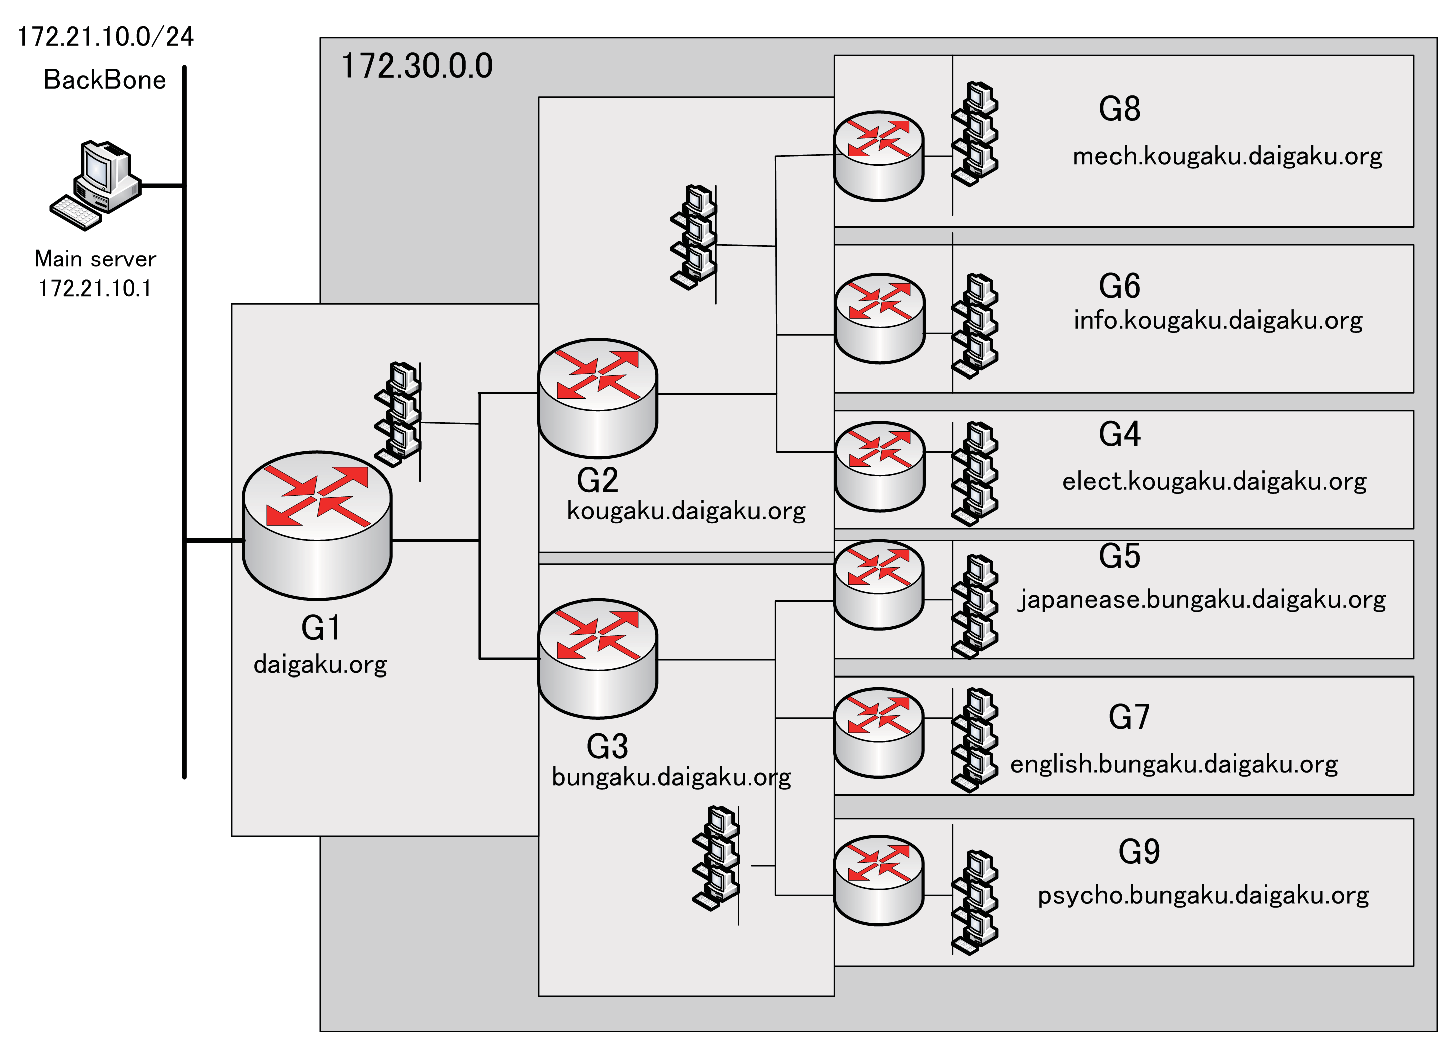
\includegraphics{./etc/specs/final.eps}}
\vspace*{-1zh}
\end{center}
\caption{最終課題構成図}
\label{final:fig:finalnet}
\end{figure}
ただし,ここで使用しているグループやドメインは仮のものであり,どのグルー
プがどこを担当し,どのようなドメイン・サブドメインにするかは後ほど決定
する.

\subsection{要求仕様}

\subsubsection{各グループのIPアドレスの割り当て}
G1以下の全体のネットワークに 172.30.0.0(ナチュラルマスク)のネットワー
クが割り当てられているので,各グループ同士で協議の上,サブネット化をし
て用いる.

\subsubsection{各グループの責任範囲}
各グループが責任を持って設定しなければならない範囲は,各グループのルー
タの上流側インターフェイスの接続・設定から下流側のサブネットワークの全
ての機器(スイッチングハブ,サーバ,コンピュータ,周辺機器,ケーブル)
である.ただし下流側ルータのインターフェイス接続は,下流側グループの担
当となる.

\subsubsection{各グループのルータのIPアドレス}
\begin{itemize}
\item 各サブネットの最も小さい IP アドレスから付与する.
\item サブネット内に複数のルータがある場合は,グループ番号の小さいものから順に付与する.
\end{itemize}

\subsubsection{ルーティング}
\begin{itemize}
\item 静的ルーティングを用いる.
\item 各ワークステーション,コンピュータ等は,デフォルトゲートウェイとして自
グループの上位側ルータを指定する.
\end{itemize}

\subsubsection{DNS ドメインの構成}
\begin{itemize}
\item G1 以下の全体ネットワークに daigaku.org ドメインが付与されている.
\item G1 が daigaku.org ゾーンを管理し,G2,G3 にそれぞれサブドメイン
  kougaku, bungaku を割り当てて,それらのゾーンを委譲する.
\item G2 は kougaku.daigaku.org ゾーンを管理し,G4,G6,G8 にそれぞれ
  elect,info,mech サブドメインを割り当て,ゾーンを委譲をする.
\item G3 は bungaku.daigaku.org ゾーンを管理し,G5,G7,G9 にそれぞれ
  japanese,english,psycho サブドメインを割り当て,ゾーンを委譲をする.
\item G4 は elect.kougaku.daigaku.org ゾーンを管理する.
\item G5 は japanese.bungaku.daigaku.org ゾーンを管理する.
\item G6 は info.kougaku.daigaku.org ゾーンを管理する.
\item G7 は english.bungaku.daigaku.org ゾーンを管理する.
\item G8 は mech.kougaku.daigaku.org ゾーンを管理する.
\item G9 は psycho.bungaku.daigaku.org ゾーンを管理する.
\item 逆引きは考えなくてよい(設定を行う必要はない).
\end{itemize}

\subsubsection{外部ネットワークとの接続}
\begin{itemize}
\item 各グループのサーバ間は,接続可能であること.
\item 各グループのサーバは,Mail server 172.21.10.1 に接続可能であること.
\item 各グループのサーバは,backbone 172.21.10.0/24 に接続可能であること.
\end{itemize}

\subsubsection{サービス}
\begin{itemize}
\item 全ての端末からメール送受信,ウェブ閲覧が行えること.
\item メールアカウントは全員分作成する.
\item その他,必要と感じるサービス,便利であると考えるサービスがあれば
  構築する.構築したサービスについては,レポートに記述すること.
\end{itemize}


\subsubsection*{考慮すべき点}
\begin{itemize}
\item どのようにネットワークの設計を行うか
\item どのような設定をして要求する仕様を満たすか.
\item ネットワークのポリシーはどのように設定すべきか.
\item 他者との共同作業をどのように行うべきか.
\item どこまでが自分の責任範囲で,どこからが他者に責任範囲か.
\item 他者への設定依頼はどのようにすべきか.
\end{itemize}


\clearpage
